\documentclass{article}%
\usepackage[T1]{fontenc}%
\usepackage[utf8]{inputenc}%
\usepackage{lmodern}%
\usepackage{textcomp}%
\usepackage{lastpage}%
\usepackage{authblk}%
\usepackage{graphicx}%
%
\title{Stac3 Inhibits Myoblast Differentiation into Myotubes}%
\author{Laura Walsh}%
\affil{Department of Oral and Maxillofacial Surgery, Hyogo College of Medicine, Nishinomiya, Hyogo 663{-}8501, Japan, Department of Genetics, Hyogo College of Medicine, Nishinomiya, Hyogo 663{-}8501, Japan}%
\date{01{-}01{-}2013}%
%
\begin{document}%
\normalsize%
\maketitle%
\section{Abstract}%
\label{sec:Abstract}%
ALBUQUERQUE, N.M. {-}{-} Around 50,000 people in New Mexico, over two{-}thirds of whom are diabetics, get HIV.\newline%
Some are diagnosed with chronic or managed maladies, and some patients have greater response to current medications than others.\newline%
And the drug therapy can be strict. Often, the medicines include either an injection and a variety of drug combinations.\newline%
Such controls made world headlines more than three years ago when researchers discovered that much faster growth of white blood cells caused by HIV infection could be accelerated by a protein called PG K{-}8.\newline%
Previous studies, funded by the National Institutes of Health, have shown an increased high clearance of HIV infection in mice.\newline%
Now, a group of scientists from the University of New Mexico Cancer Center has published findings suggesting PG K{-}8 also may be potent neurotoxin in humans.\newline%
Reporting in the journal Nature Genetics, the team, led by Serguei Cosniotis, professor of developmental biology at the University of New Mexico, and colleagues, says the protein reveals more about how the immune system react to HIV infection and what it means for the risk of complications from HIV.\newline%
Cosniotis said he originally treated his patients with a gold standard drug therapy called infliximab. But after a team discovered that glycolysis was more of a bad player than the other three drugs combined, he and his colleagues decided to change the focus of the therapy to PG K{-}8.\newline%
He said their aim was to find a way to distribute the prevention drug so people who are also genetically predisposed to HIV infection would get high clearance of the virus.\newline%
Likely persons of concern would be those genetically predisposed to getting HIV, Cosniotis said.\newline%
But recipients in the study, who included HIV patients and those with a less than normal genetic make{-}up, displayed significantly increased levels of (beta{-}methylpfantone{-}gases) which build up when the immune system works on the cell.\newline%
The researchers also found a transcription factor called RNA{-}Fop3 is more than 40 times more potent for the synthesis of the neurotoxin in laboratory animals.\newline%
Cosniotis said natural production of RNA{-}Fop3 was put on hold so only one of the protein's key proteins was found in human cells.\newline%
But the anti{-}neptune and protective action of the antioxidant beta{-}oxygen (EOG) "is fully suppressed" in humans when stimulated by the protein, he said.\newline%
"The behavioral and molecular changes we observed by PG K{-}8 in mice with chronic HIV infection with EOG are consistent with the toxicity profile of the lead product," Cosniotis said.\newline%
While current chemists are working on a new formulation of EOG, Cosniotis said the work was promising.\newline%
He said the strategy offers a real option that could be used to keep the HIV virus at bay.\newline%
The New Mexico researchers also plan to look for other protective substances, including "from the other 'fists,' the Maternoid acid mucosal leukocyte, on the individuals most exposed to cytotoxic effects of EOG."

%
\subsection{Image Analysis}%
\label{subsec:ImageAnalysis}%


\begin{figure}[h!]%
\centering%
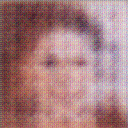
\includegraphics[width=150px]{500_fake_images/samples_5_295.png}%
\caption{A Close Up Of A Person Holding A Toothbrush}%
\end{figure}

%
\end{document}